
\tikzset{every picture/.style={line width=0.75pt}} %set default line width to 0.75pt        

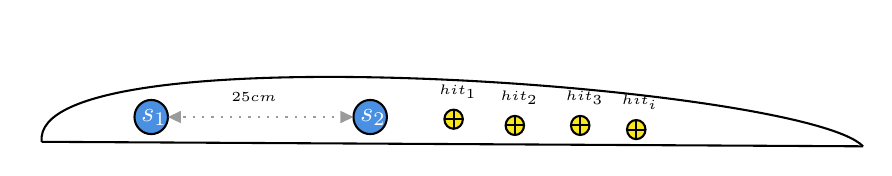
\begin{tikzpicture}[x=0.75pt,y=0.75pt,yscale=-1,xscale=1]
%uncomment if require: \path (0,300); %set diagram left start at 0, and has height of 300

%Curve Lines [id:da37291442444066547] 
\draw    (57,87) .. controls (50.74,32.51) and (424.54,59.84) .. (452.74,89.17) ;
%Straight Lines [id:da5213498635173044] 
\draw    (57,87) -- (452.74,89.17) ;
%Shape: Ellipse [id:dp5451517635936938] 
\draw  [color={rgb, 255:red, 0; green, 0; blue, 0 }  ,draw opacity=1 ][fill={rgb, 255:red, 74; green, 144; blue, 226 }  ,fill opacity=1 ] (101.7,75.06) .. controls (101.7,70.51) and (105.31,66.83) .. (109.76,66.83) .. controls (114.21,66.83) and (117.82,70.51) .. (117.82,75.06) .. controls (117.82,79.6) and (114.21,83.28) .. (109.76,83.28) .. controls (105.31,83.28) and (101.7,79.6) .. (101.7,75.06) -- cycle ;
\draw  [fill={rgb, 255:red, 248; green, 231; blue, 28 }  ,fill opacity=1 ] (251,76.11) .. controls (251,73.56) and (253,71.5) .. (255.46,71.5) .. controls (257.92,71.5) and (259.91,73.56) .. (259.91,76.11) .. controls (259.91,78.65) and (257.92,80.72) .. (255.46,80.72) .. controls (253,80.72) and (251,78.65) .. (251,76.11) -- cycle ; \draw   (251,76.11) -- (259.91,76.11) ; \draw   (255.46,71.5) -- (255.46,80.72) ;
%Shape: Ellipse [id:dp5239731363628557] 
\draw  [color={rgb, 255:red, 0; green, 0; blue, 0 }  ,draw opacity=1 ][fill={rgb, 255:red, 74; green, 144; blue, 226 }  ,fill opacity=1 ] (207.2,75.06) .. controls (207.2,70.51) and (210.81,66.83) .. (215.26,66.83) .. controls (219.71,66.83) and (223.32,70.51) .. (223.32,75.06) .. controls (223.32,79.6) and (219.71,83.28) .. (215.26,83.28) .. controls (210.81,83.28) and (207.2,79.6) .. (207.2,75.06) -- cycle ;
%Straight Lines [id:da7318958622897511] 
\draw [color={rgb, 255:red, 155; green, 155; blue, 155 }  ,draw opacity=1 ] [dash pattern={on 0.84pt off 2.51pt}]  (120.82,75.06) -- (204.2,75.06) ;
\draw [shift={(207.2,75.06)}, rotate = 180] [fill={rgb, 255:red, 155; green, 155; blue, 155 }  ,fill opacity=1 ][line width=0.08]  [draw opacity=0] (6.25,-3) -- (0,0) -- (6.25,3) -- cycle    ;
\draw [shift={(117.82,75.06)}, rotate = 0] [fill={rgb, 255:red, 155; green, 155; blue, 155 }  ,fill opacity=1 ][line width=0.08]  [draw opacity=0] (6.25,-3) -- (0,0) -- (6.25,3) -- cycle    ;
\draw  [fill={rgb, 255:red, 248; green, 231; blue, 28 }  ,fill opacity=1 ] (280.5,79.11) .. controls (280.5,76.56) and (282.5,74.5) .. (284.96,74.5) .. controls (287.42,74.5) and (289.41,76.56) .. (289.41,79.11) .. controls (289.41,81.65) and (287.42,83.72) .. (284.96,83.72) .. controls (282.5,83.72) and (280.5,81.65) .. (280.5,79.11) -- cycle ; \draw   (280.5,79.11) -- (289.41,79.11) ; \draw   (284.96,74.5) -- (284.96,83.72) ;
\draw  [fill={rgb, 255:red, 248; green, 231; blue, 28 }  ,fill opacity=1 ] (312,79.11) .. controls (312,76.56) and (314,74.5) .. (316.46,74.5) .. controls (318.92,74.5) and (320.91,76.56) .. (320.91,79.11) .. controls (320.91,81.65) and (318.92,83.72) .. (316.46,83.72) .. controls (314,83.72) and (312,81.65) .. (312,79.11) -- cycle ; \draw   (312,79.11) -- (320.91,79.11) ; \draw   (316.46,74.5) -- (316.46,83.72) ;
\draw  [fill={rgb, 255:red, 248; green, 231; blue, 28 }  ,fill opacity=1 ] (339,81.11) .. controls (339,78.56) and (341,76.5) .. (343.46,76.5) .. controls (345.92,76.5) and (347.91,78.56) .. (347.91,81.11) .. controls (347.91,83.65) and (345.92,85.72) .. (343.46,85.72) .. controls (341,85.72) and (339,83.65) .. (339,81.11) -- cycle ; \draw   (339,81.11) -- (347.91,81.11) ; \draw   (343.46,76.5) -- (343.46,85.72) ;

% Text Node
\draw (103.56,69.94) node [anchor=north west][inner sep=0.75pt]  [color={rgb, 255:red, 255; green, 255; blue, 255 }  ,opacity=1 ] [align=left] {$\displaystyle s_{1}$};
% Text Node
\draw (209.06,69.94) node [anchor=north west][inner sep=0.75pt]  [color={rgb, 255:red, 255; green, 255; blue, 255 }  ,opacity=1 ] [align=left] {$\displaystyle s_{2}$};
% Text Node
\draw (147,62) node [anchor=north west][inner sep=0.75pt]  [font=\tiny] [align=left] {$\displaystyle 25cm\ $};
% Text Node
\draw (247.06,57.94) node [anchor=north west][inner sep=0.75pt]  [font=\tiny,color={rgb, 255:red, 0; green, 0; blue, 0 }  ,opacity=1 ] [align=left] {$\displaystyle hit_{1}$};
% Text Node
\draw (276.56,60.94) node [anchor=north west][inner sep=0.75pt]  [font=\tiny,color={rgb, 255:red, 0; green, 0; blue, 0 }  ,opacity=1 ] [align=left] {$\displaystyle hit_{2}$};
% Text Node
\draw (308.06,60.94) node [anchor=north west][inner sep=0.75pt]  [font=\tiny,color={rgb, 255:red, 0; green, 0; blue, 0 }  ,opacity=1 ] [align=left] {$\displaystyle hit_{3}$};
% Text Node
\draw (335.06,62.94) node [anchor=north west][inner sep=0.75pt]  [font=\tiny,color={rgb, 255:red, 0; green, 0; blue, 0 }  ,opacity=1 ] [align=left] {$\displaystyle hit_{i}$};


\end{tikzpicture}